\section{Simulation}\label{sec:simulation}
This section documents the Monte Carlo simulation results for the HAL-MLE. We (i) test the uniform convergence and pointwise asymptotic normality of the HAL-MLE, (ii) test the asymptotic efficiency of the plug-in HAL-MLE and HAL-TMLE, and (iii) compare it with the logspline, TF and its equivalent variant with penalty on the parametric part (TFPP), and KDE methods, over a vast range of different DGPs and sample sizes.

\subsection{DGPs}
We use six univariate densities on $[0,1]$ across continuous vs discrete, concentrated vs heavy-tailed, and smooth vs oscillatory (single-scale vs multi-scale). The six DGPs are: Truncated Normal (TN), Truncated GMM with three equally spaced modes (GS3), Truncated GMM with three modes of differing scales and weights (GA3), Truncated GMM with five spikes and background (GS5), Step Function (Step), and Sinusoidal (Sine), as shown in Figure~\ref{fig:dgps}. We provide the ground–truth density $p_0$ and population parameters, like moments, median, etc. in Appendix~\ref{app:dgp_setup}.

\begin{figure}[H]
    \centering
    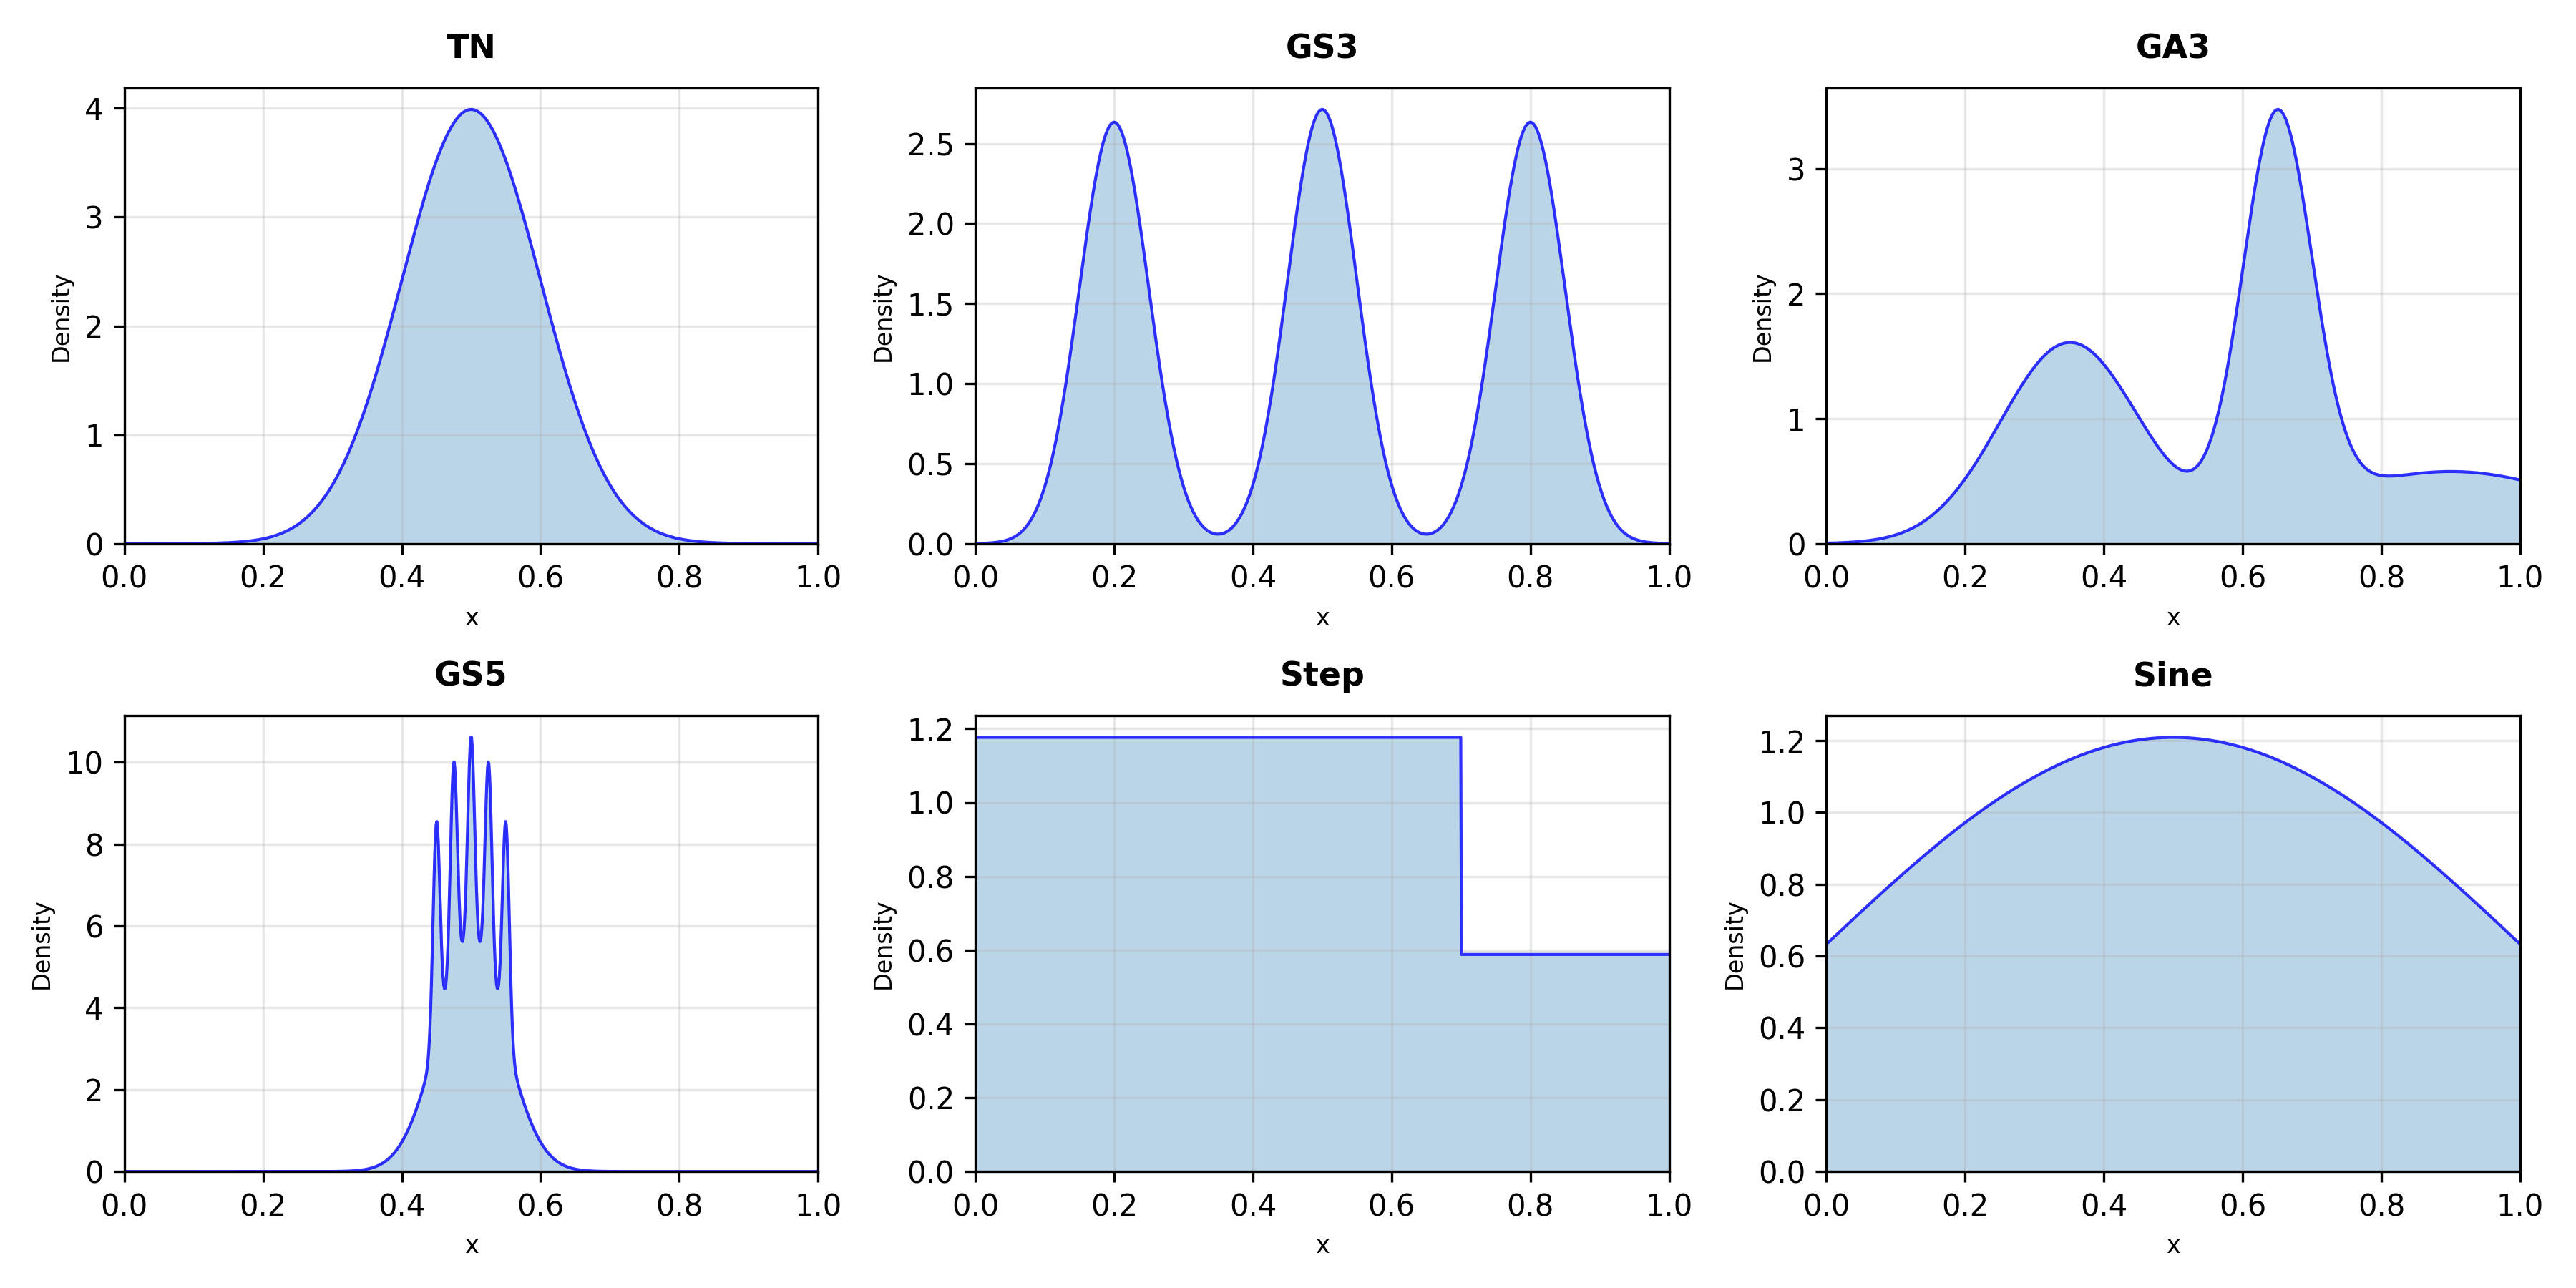
\includegraphics[width=0.9\textwidth]{resources/simulation_dgp.png}
    \caption{Six DGPs: (a) TN, (b) GS3, (c) GA3, (d) GS5, (e) Step, (f) Sine.}
    \label{fig:dgps}
\end{figure}


\subsection{Implementation of Cross-Validation with Optuna}
We use a 5-fold cross-validation to cross validate over the $L_1$ norm constraint and the basis order of the HAL-MLE. Instead of cross validating over each grid of the hyperparameter pairs, we used Optuna \citep{akiba2019optuna} to sample the hyperparameters with 50 steps. Throughout the cross-validation steps, we acknowledge the failure of the solvers occasionally and we have to switch to other solvers in \texttt{CVXPY}. In general, \texttt{MOSEK} is the fastest solver, and we use it as the default solver. \texttt{SCS} is relatively slow but more robust. The search space is $L_1$ norm constraint in $[10^{-3},10^{6}]$ (log scale) and basis order in $\{0,1,2\}$. The trial budget is 50 evaluations per estimator/DGP/sample size. As claimed in \citep{akiba2019optuna}, the performance of Optuna is very close to the performance of the grid search with a massive reduction in computational cost.

\subsection{HAL-MLE density estimation}
We here demonstrate the uniform convergence and pointwise asymptotic normality of the HAL-MLE.

\subsubsection{Uniform convergence (sup\textendash norm error)} \label{subsec:simulation_uniform_convergence}
We consider eight sample sizes, from $n=25$ to $n=3200$, with $1000$ independent random samples per DGP at each $n$. For each sample, we approximate the sup\textendash norm error $\lVert p_{f_n} - p_0 \rVert_{\infty}$ by evaluating both the estimator and the truth on a uniform grid of 201 points over $[0,1]$ and taking the maximum absolute deviation over grid points. By Theorem~\ref{thm:uniform-density-hal}, the uniform convergence rate is $O_p^+\big(n^{-(k+1)/(2k+3)}\big)$ for basis order $k\in\{1,2\}$. Because $k$ is selected by cross-validation over this set, we expect at least $O_p\big(n^{-1/3}\big)$ decay, even though we do not have the uniform convergence rate for $k = 0$. This can be read off from the median lines of the boxplots below as $n$ increases. If there is a convergence rate, the median line should be approximately a straight line with a decreasing slope, expected to be around or above $-\frac13$. 

We aggregate errors across samples and summarize their distributions by sample size using boxplots (both linear\textendash and log\textendash scale). The results for each DGPs are shown below in Figure~\ref{fig:uniform_convergence}.

\begin{figure}[H]
    \centering
    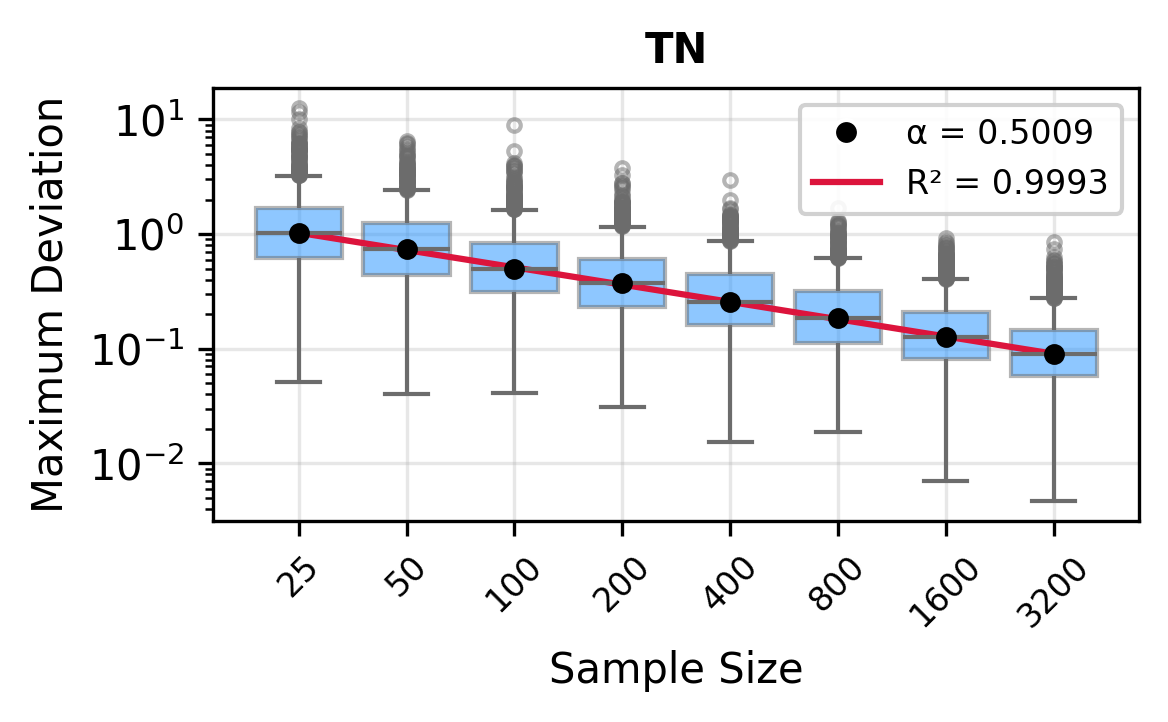
\includegraphics[width=.32\textwidth]{resources/density_uniform_convergence/uniform_convergence_truncatednormal_cvxpy_log.png}
    \hfill
    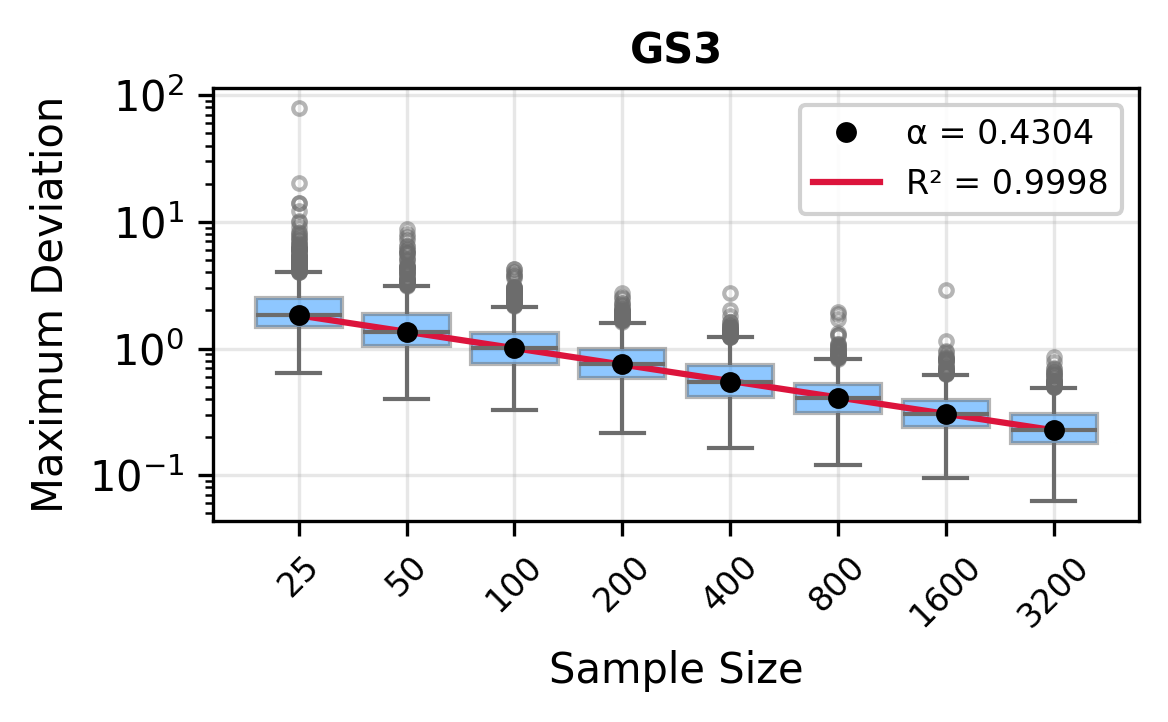
\includegraphics[width=.32\textwidth]{resources/density_uniform_convergence/uniform_convergence_truncatedgmmsymmetricthree_cvxpy_log.png}
    \hfill
    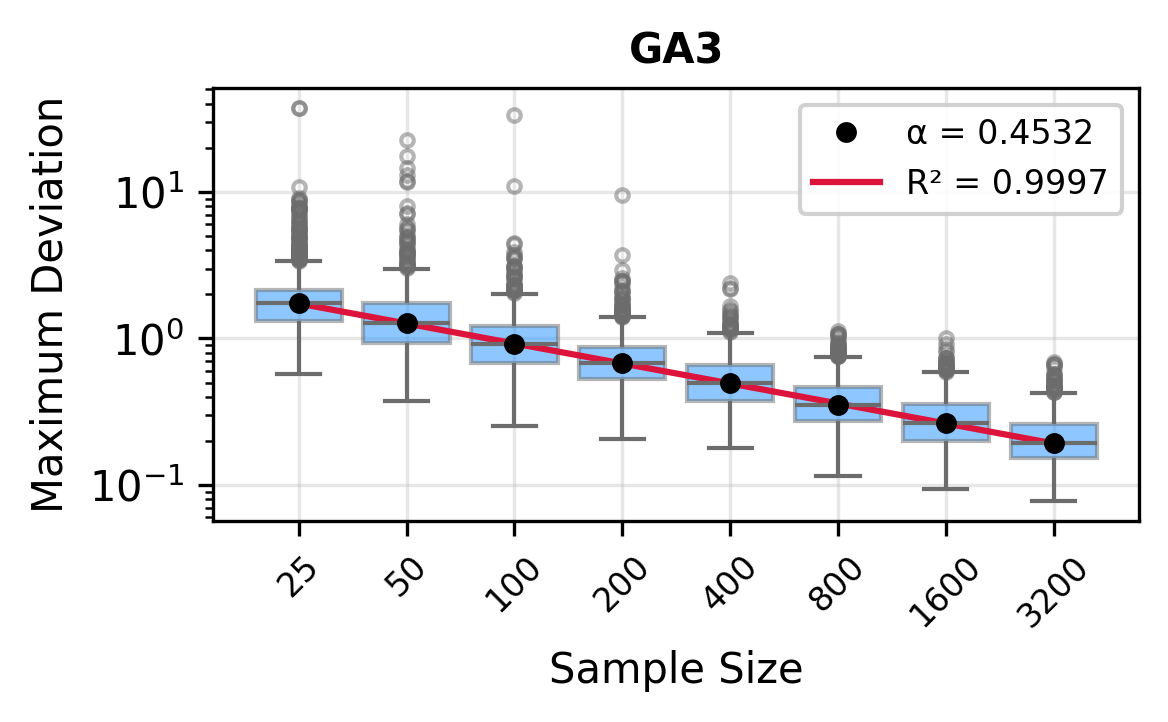
\includegraphics[width=.32\textwidth]{resources/density_uniform_convergence/uniform_convergence_truncatedgmmasymmetricthree_cvxpy_log.png}

    \vspace{0.4em}

    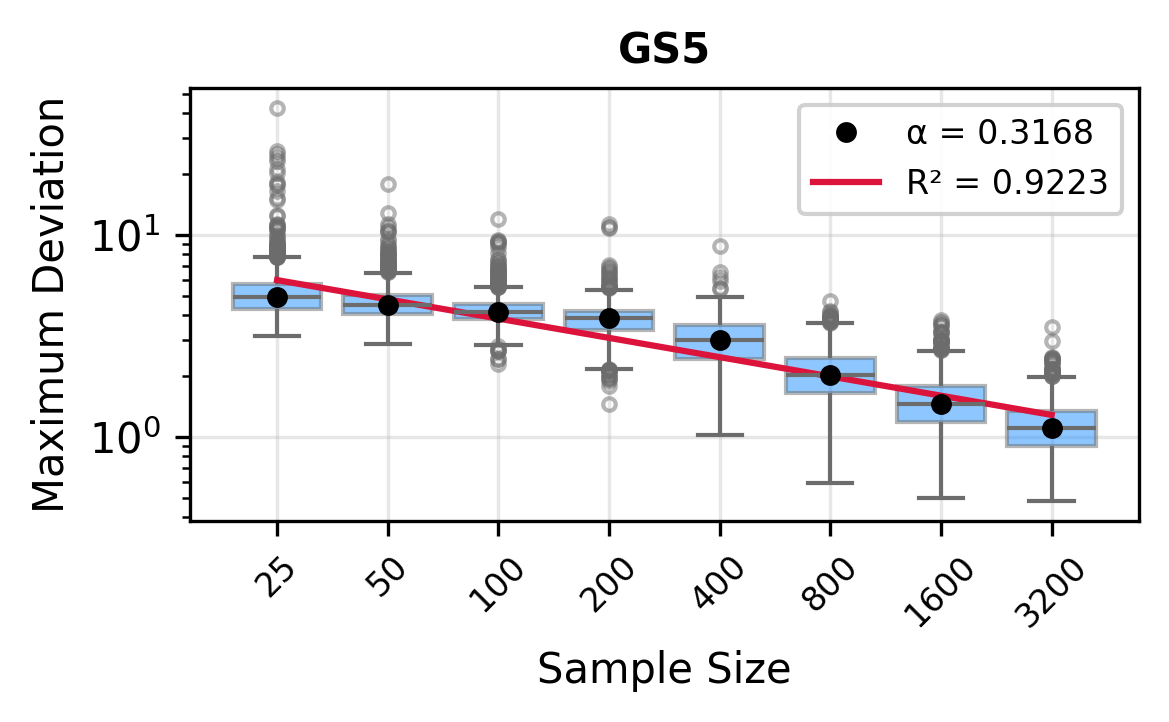
\includegraphics[width=.32\textwidth]{resources/density_uniform_convergence/uniform_convergence_truncatedgmmfivespikes_cvxpy_log.png}
    \hfill
    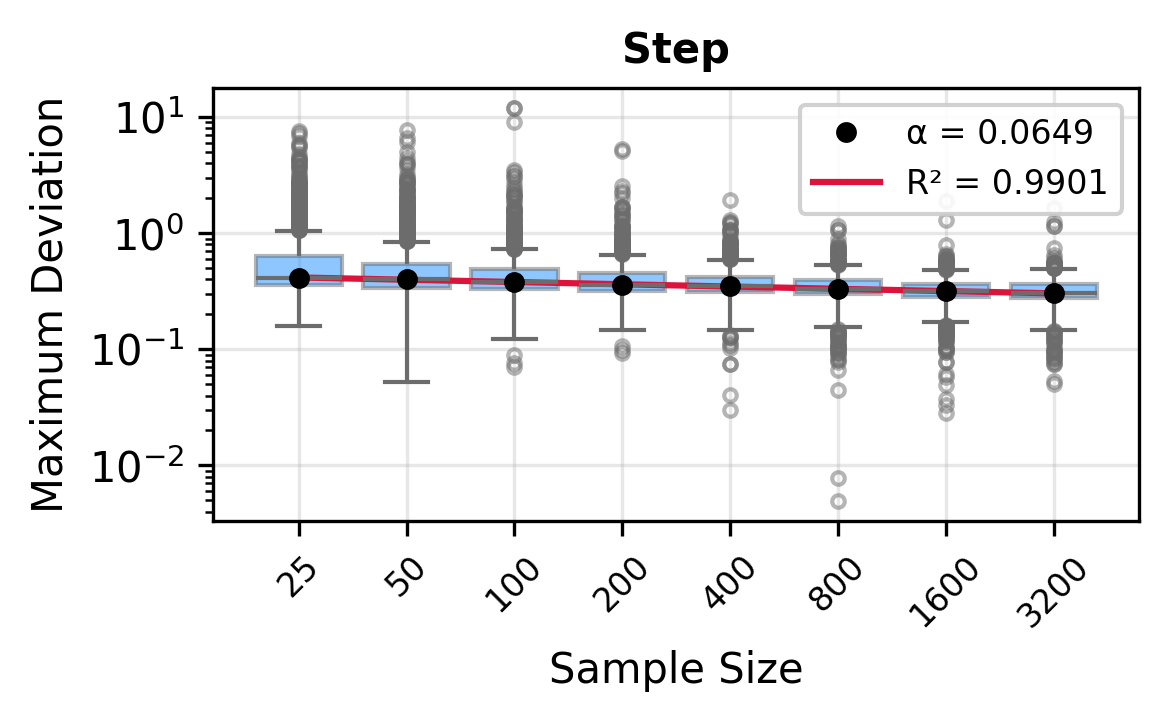
\includegraphics[width=.32\textwidth]{resources/density_uniform_convergence/uniform_convergence_stepfunction_cvxpy_log.png}
    \hfill
    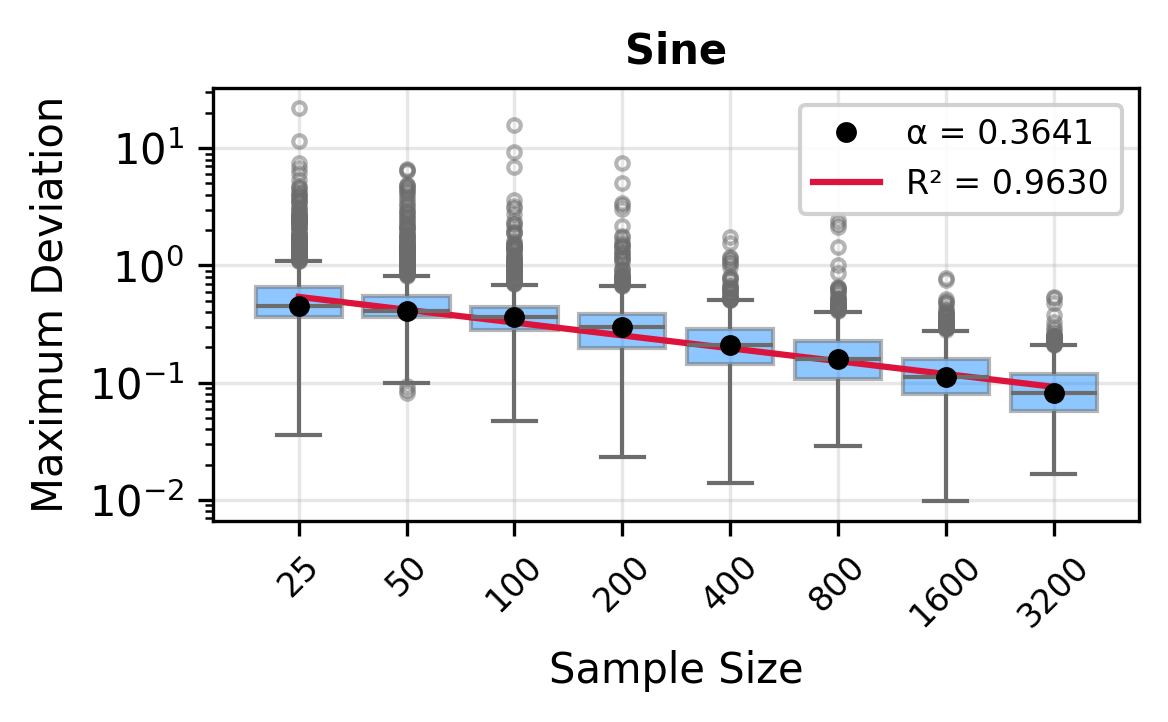
\includegraphics[width=.32\textwidth]{resources/density_uniform_convergence/uniform_convergence_sinusoidal_cvxpy_log.png}
    \caption{Uniform\textendash convergence sup\textendash norm error (log\textendash scale) by DGP. Panels (row\textendash wise, left to right): (a) TN, (b) GS3, (c) GA3, (d) GS5, (e) Step, (f) Sine.}
    \label{fig:uniform_convergence}
\end{figure}

We regress the median error on the sample size on a log-log scale and report the slope and $R^2$ in Table~\ref{tab:uniform_convergence_scaling}. The results are shown below in Table~\ref{tab:uniform_convergence_scaling}.

% Auto-generated scaling law summary table
% Auto-generated scaling law summary table
\begin{table}[H]
  \centering
  \small
  \setlength{\tabcolsep}{4pt}
  \renewcommand{\arraystretch}{1.2}
  \begin{tabular}{lcccccc}
    \toprule
    Metric & TN & GS3 & GA3 & GS5 & Step & Sine \\
    \midrule
    $\alpha$ (Decay Exponent) & 0.5009 & 0.4304 & 0.4532 & 0.3168 & 0.0649 & 0.3641 \\
    $R^2$ (Goodness of Fit) & 0.9993 & 0.9998 & 0.9997 & 0.9223 & 0.9901 & 0.9630 \\
    Significant ($p < 0.05$) & Yes & Yes & Yes & Yes & Yes & Yes \\
    \bottomrule
  \end{tabular}
  \caption{Uniform convergence scaling analysis. $\alpha$ represents the decay exponent in the power law $\text{error} \propto n^{-\alpha}$. $R^2$ measures goodness of fit on the log-log scale. Significance tests $H_0: \text{slope} = 0$ vs $H_1: \text{slope} \neq 0$ at $\alpha = 0.05$.}
  \label{tab:uniform_convergence_scaling}
\end{table}

This Table~\ref{tab:uniform_convergence_scaling} verifies that the adaptive HAL-MLE that selects the smoothness $k$ with cross-validation is converging at an adaptive rate. And the adaptive rates we are seeing align with the  smoothness of the DGPs. The Step Function might be too easy and does not have a huge space for improvement.

\subsubsection{Asymptotic normality: pointwise SE, CI width, and coverage.} \label{subsec:simulation_asymptotic_normality}
We assess the pointwise asymptotic normality of the HAL-MLE density mentioned in Theorem~\ref{thm:density_HAL_asymptotic_normality} and evaluate the performance of density variance estimation via the delta-method in Eq.~\ref{eq:delta-method-variance-estimator}. We assess the density variance estimation performance by introducing the oracle CI, which is the HAL-MLE point estimate \(\pm 1.96\) times the empirical standard deviation of the fitted densities across 1000 samples. Then, we evaluate the variance estimator by computing the coverage of the CI constructed by the z-statistic of the HAL-MLE point estimate. 

For each DGP and sample size \(n\), we evaluate on the 201 grid points between the first and last observation and summarize (i) interval widths and (ii) coverage of the truth \(p_0(x)\). Coverage is computed pointwise as the fraction of replicates whose 95\% CI contains the truth at each grid point. The coverage of the Delta-method variance estimator is the mean coverage over the 201 grid points. The full results, including the CI widths and the coverage of each grid point, are included in Appendix~\ref{app_i_subsec:asymptotic_normality_and_var_est}.
% \begin{figure}[H]
%     \centering
%     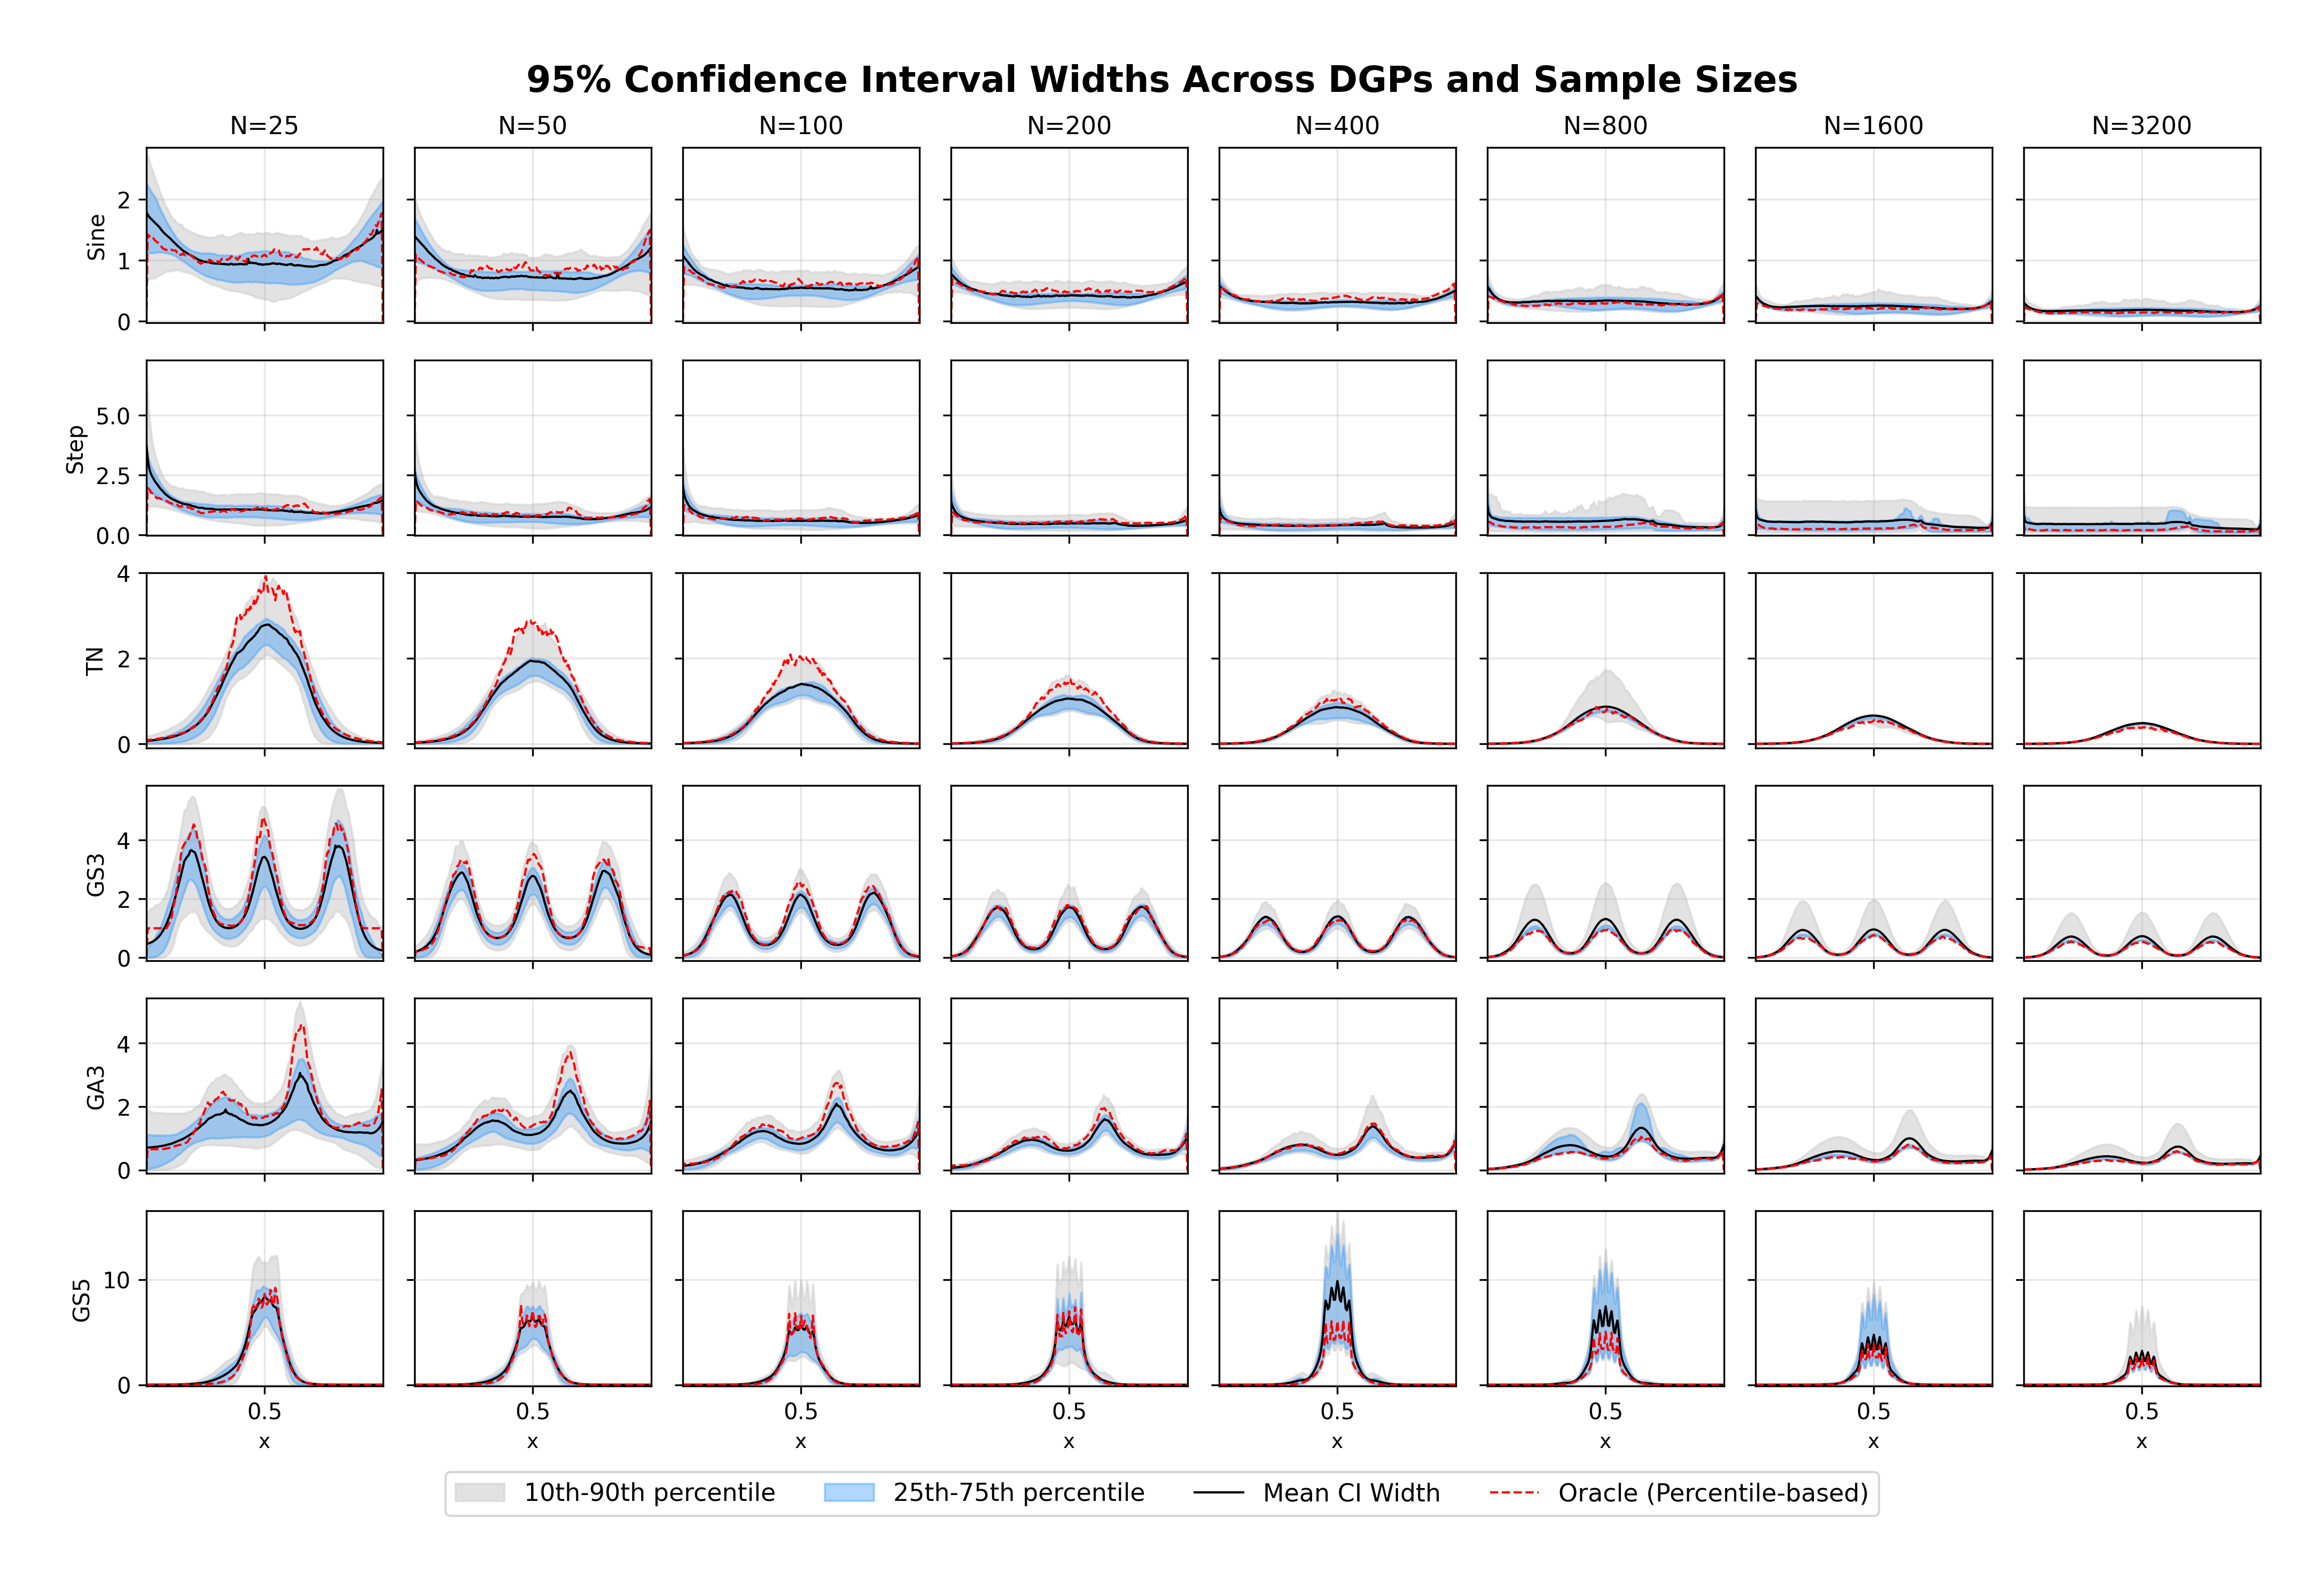
\includegraphics[width=\textwidth]{resources/density_asymptotic_normality_and_var_est/Figure_CI_Widths_Combined.png}
%     \caption{Pointwise 95\% CI widths for HAL\textendash MLE across DGPs (rows) and sample sizes (columns). Shaded bands show the 10\%--90\% (light gray) and 25\%--75\% (blue) percentiles over replicates; the black line is the mean width. The red dashed line overlays the oracle percentile width.}
%     \label{fig:ci-widths}
% \end{figure}

\noindent Table~\ref{tab:coverage_analysis} reports mean coverage summaries by DGP and sample size, shown as (plug\textendash in, oracle). Abbreviations: TN, GS3/GA3, GS5, Step, Sine. Each cell shows (estimated coverage, oracle coverage). Oracle coverage uses the empirical standard deviation across Monte Carlo Simulations.

% Auto-generated coverage analysis table
\begin{table}[H]
  \centering
  \scriptsize
  \setlength{\tabcolsep}{2pt}
  \renewcommand{\arraystretch}{1.1}
  \begin{tabular}{lcccccccc}
    \toprule
    DGP & N=25 & N=50 & N=100 & N=200 & N=400 & N=800 & N=1600 & N=3200 \\
    \midrule
    TN & (94.7, 93.6) & (93.8, 92.9) & (93.7, 93.2) & (93.7, 92.1) & (92.6, 92.2) & (95.1, 92.1) & (95.5, 92.2) & (91.2, 92.0) \\
    GS3 & (83.7, 90.9) & (89.9, 91.2) & (90.0, 90.8) & (90.5, 91.3) & (91.2, 91.1) & (93.3, 91.4) & (92.2, 91.4) & (91.7, 91.4) \\
    GA3 & (81.5, 91.9) & (85.2, 92.4) & (87.7, 92.6) & (88.6, 92.9) & (90.9, 92.9) & (94.9, 92.8) & (95.6, 92.6) & (95.2, 92.8) \\
    GS5 & (93.8, 95.4) & (91.2, 94.1) & (88.9, 92.7) & (90.4, 93.7) & (95.3, 96.5) & (95.6, 96.5) & (94.5, 96.6) & (94.7, 96.4) \\
    Step & (90.0, 94.2) & (85.9, 92.2) & (81.9, 90.6) & (80.3, 90.3) & (82.9, 90.0) & (90.0, 90.1) & (93.2, 90.5) & (94.2, 91.0) \\
    Sine & (92.5, 94.3) & (91.0, 94.4) & (88.5, 94.7) & (85.5, 94.1) & (89.5, 92.8) & (94.2, 93.5) & (95.9, 93.5) & (96.2, 93.5) \\
    \bottomrule
  \end{tabular}
  \caption{Coverage probabilities (\%) for 95\% confidence intervals across DGPs and sample sizes.}
  \label{tab:coverage_analysis}
\end{table}

We can see that the oracle CI coverage is always around 95\%, which means the density estimation is pointwise asymptotically normal. For most of the DGPs, the Delta-method variance estimator is also very close to the oracle CI coverage. A limitation of the Delta-method is that it does not work as well on the extrapolated region, where we have no data. For example, in the GS5 DGP, the distribution is very concentrated and the data points are centered around [0.2,0.8]. And the Delta-method variance estimator is not working as well when testing the coverage on the margins, even though the density estimation is still asymptotically normal.

\subsubsection{Asymptotic efficiency of plug-in HAL-MLE and HAL-TMLE.} \label{subsec:simulation_asymptotic_efficiency_of_plug_in_hal_mle_and_hal_tmle}
We here evaluate the asymptotic efficiency of the plug-in HAL-MLE and HAL-TMLE by comparing their performance in estimating some statistical estimands such as the mean, median, survival at 0.5, and second moment, against the existing asymptotically efficient estimators.

Trivially, the asymptotically efficient estimator of the population mean is the sample mean. And the asymptotically efficient estimator of the population median is the sample median. The asymptotically efficient estimator of population survival probability at 0.5 is the empirical survival proportion at 0.5. The asymptotically efficient estimator of the population second moment is the sample second moment.

Across DGPs and sample sizes, we compare the bias, variance, MSE, and the ratio bias/sd of plug-in HAL-MLE and HAL-TMLE with the asymptotically efficient estimators. The results of GA3 are shown below in Figure~\ref{fig:efficiency-comparison-ga3}. The full results are included in Appendix~\ref{app_i_subsec:asymptotic_efficiency}.

\begin{figure}[H]
  \centering
  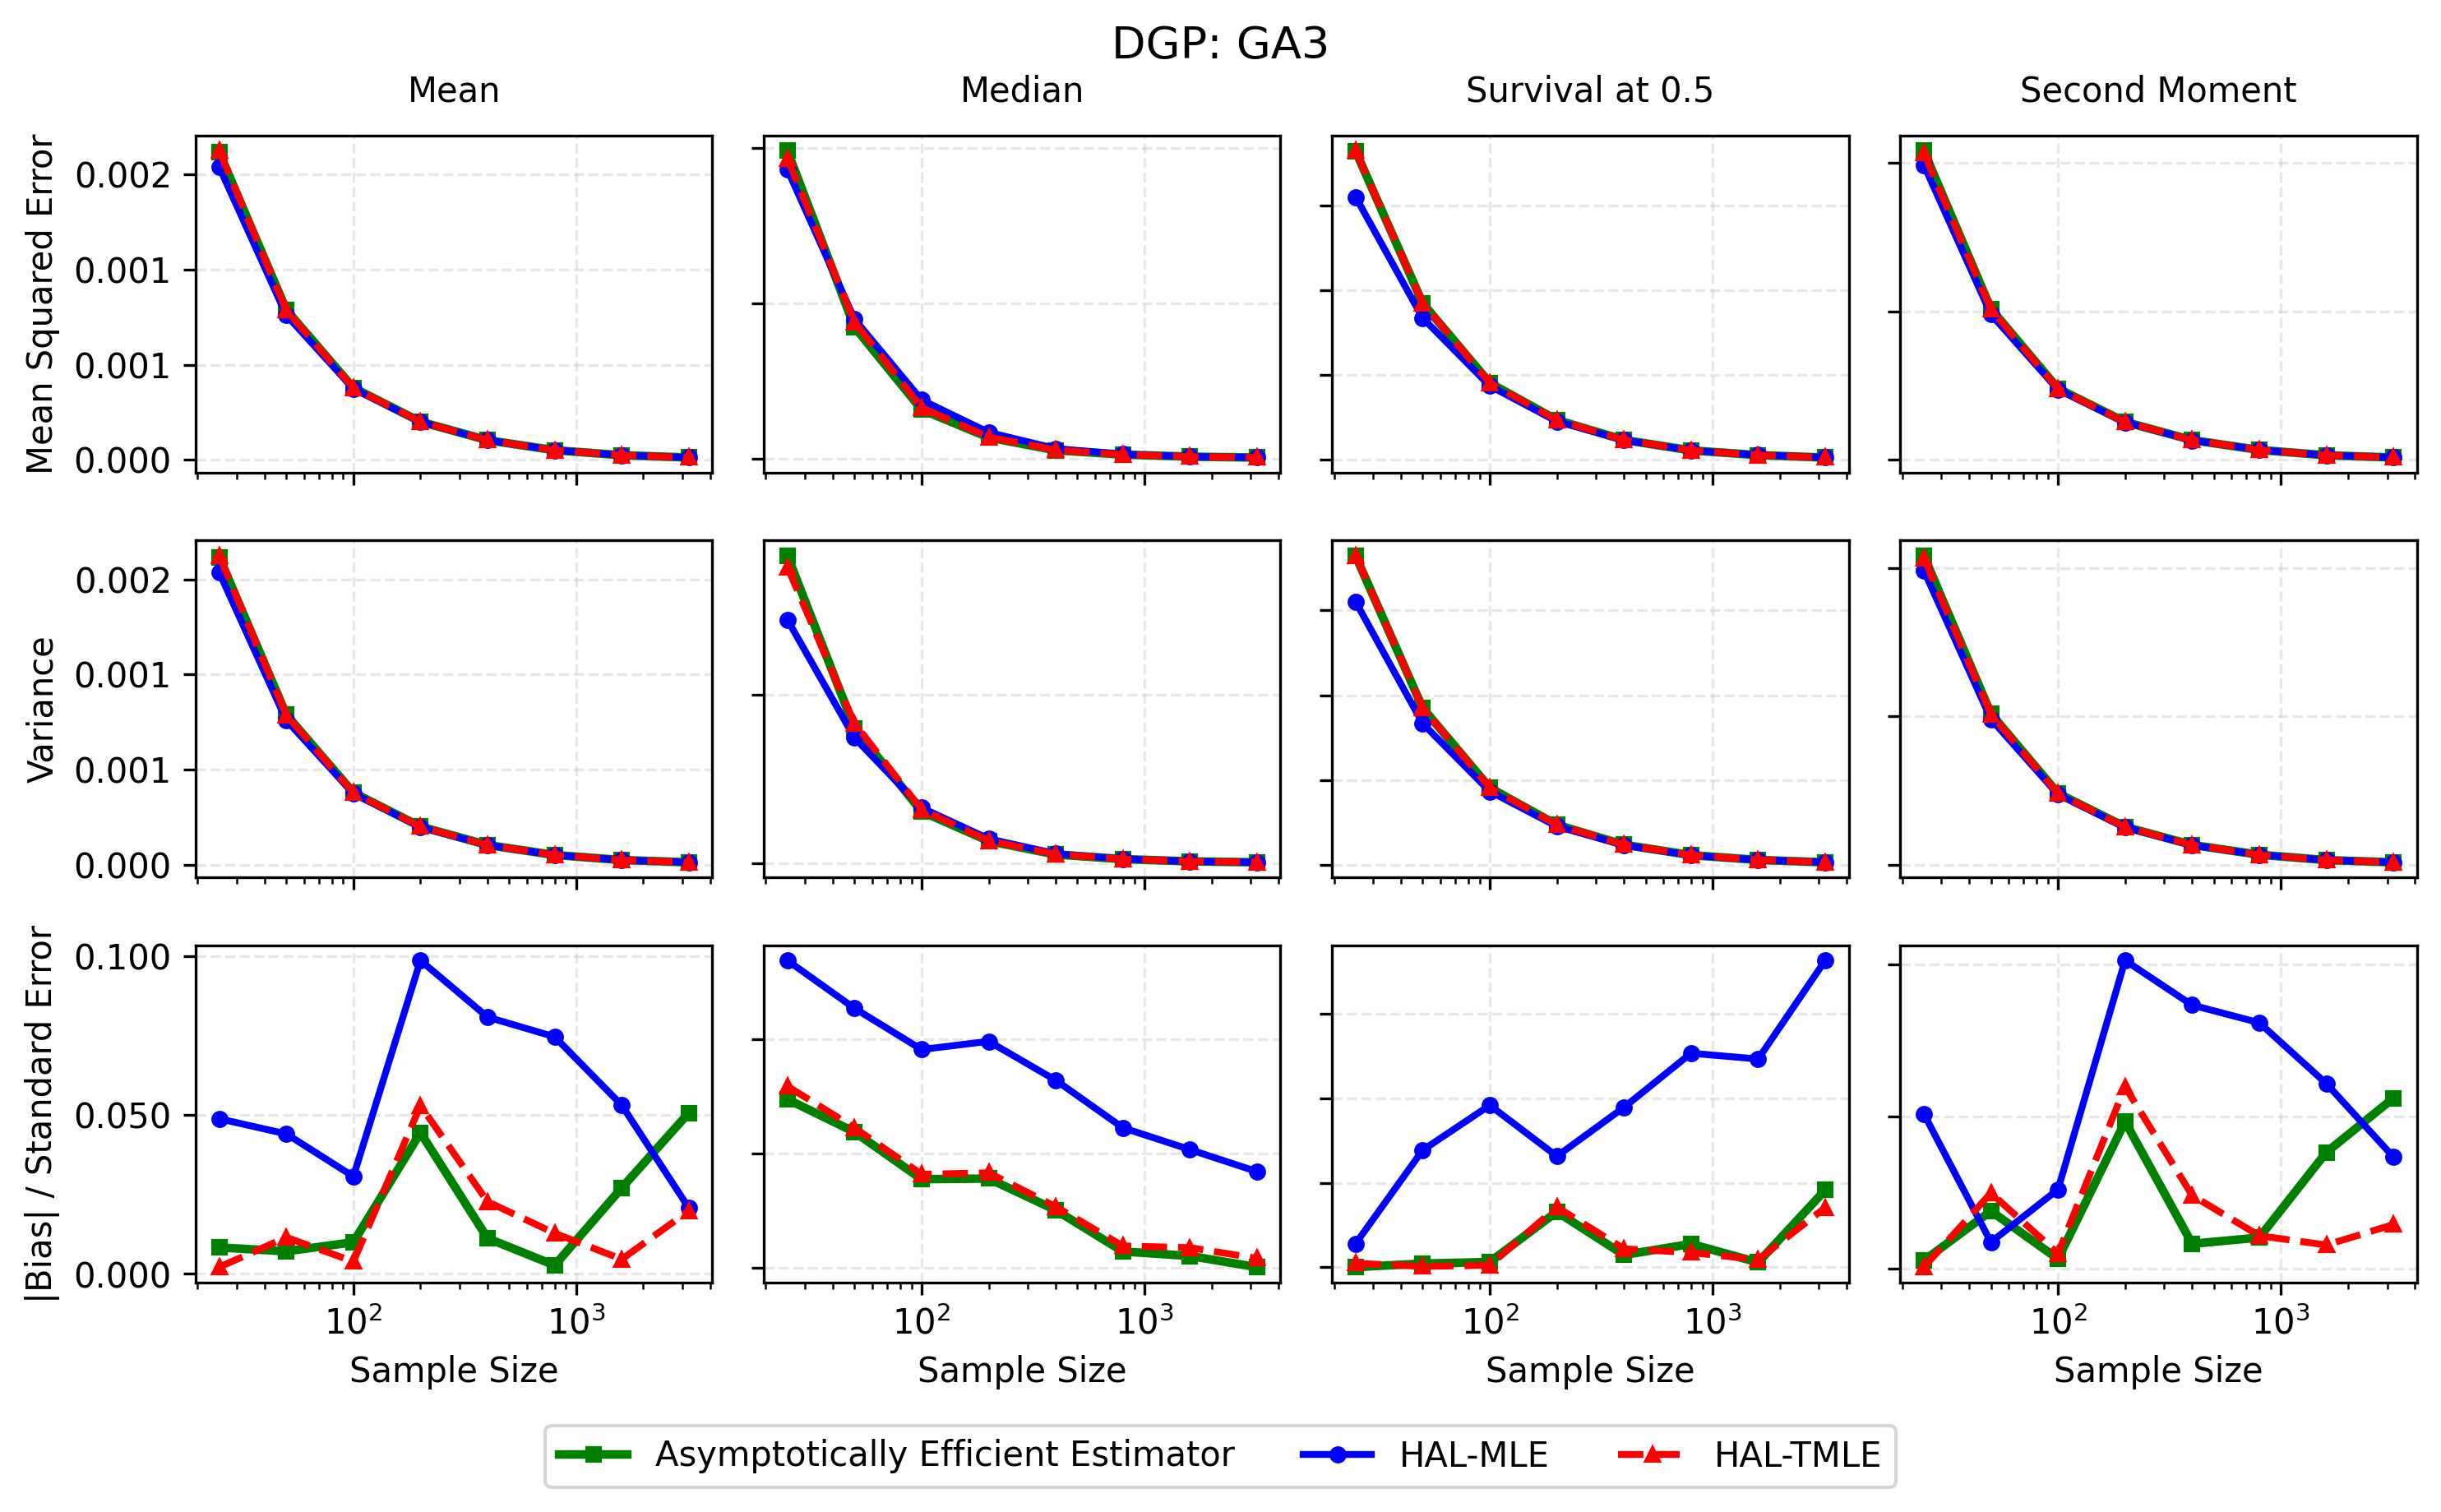
\includegraphics[width=\textwidth]{resources/density_asymptotic_efficiency/TruncatedGMMAsymmetricThree/efficiency_comparison.png}
  \caption{Representative asymptotic\textendash efficiency comparison (DGP: GA3). Columns show four statistical estimands (Mean, Median, Survival at 0.5, Second Moment) and rows show three metrics (MSE, Variance, $|$Bias$|$/SE). Curves compare the asymptotically efficient estimator (green), HAL\textendash MLE (blue), and HAL\textendash TMLE (red).}
  \label{fig:efficiency-comparison-ga3}
\end{figure}

They are comparable and thus verify the asymptotic efficiency of the plug-in HAL-MLE and HAL-TMLE. We can see that sometimes the plug-in HAL-MLE has super-efficiency over the asymptotically efficient estimator when the sample size is small. But after targeting, the EIC equation is solved, and the HAL-TMLE performance is the same as the asymptotically efficient estimator uptill some numerical errors. In the univariate case, we cannot expect the performance of Plug-in HAL-MLE and HAL-TMLE to be significantly better than their corresponding asymptotic efficient estimators, but one major advantage is that we can provide nonparametric inference using the EIC-based confidence interval.

\subsection{EIC\textendash based variance estimation for statistical estimands.} \label{subsec:simulation_eic-based-variance-estimation}
We evaluate the EIC-based variance estimation introduced in Section~\ref{subsec: EIC-based-variance-estimation} for the statistical estimands by computing the plug-in standard errors via the efficient influence curve and comparing the coverage of the oracle. We report the coverage of the 95\% confidence interval for four estimands—mean, second moment, survival at 0.5, and median—across six DGPs and eight sample sizes in Tables~\ref{tab:coverage_targeting_mean}, \ref{tab:coverage_targeting_second_moment}, \ref{tab:coverage_targeting_survival_0_5}, and \ref{tab:coverage_targeting_median}. Each table shows, for every DGP and sample size, the pair (EIC-based coverage, oracle coverage). EIC-based coverage uses plug-in standard errors derived from the efficient influence curve, while oracle coverage uses the empirical standard deviation of estimates across Monte Carlo simulations.


The full figure panels of CI width and coverage for each DGP are provided in Appendix~\ref{app_i_subsec:eic-based-variance-estimation}.

% Auto-generated targeting coverage analysis table
\begin{table}[H]
  \centering
  \scriptsize
  \setlength{\tabcolsep}{2pt}
  \renewcommand{\arraystretch}{1.1}
  \begin{tabular}{lcccccccc}
    \toprule
    DGP & N=25 & N=50 & N=100 & N=200 & N=400 & N=800 & N=1600 & N=3200 \\
    \midrule
    TN & (93.3, 94.6) & (94.4, 96.0) & (94.9, 95.2) & (95.8, 95.4) & (94.7, 94.7) & (93.9, 95.1) & (95.3, 95.2) & (94.3, 94.3) \\
    GS3 & (95.1, 95.9) & (95.2, 95.8) & (95.7, 95.9) & (95.5, 94.9) & (94.3, 95.1) & (95.3, 94.9) & (95.1, 94.6) & (96.3, 96.1) \\
    GA3 & (94.8, 95.4) & (94.7, 95.3) & (95.6, 94.6) & (95.3, 95.0) & (94.9, 95.2) & (94.3, 94.2) & (96.2, 94.9) & (94.8, 94.6) \\
    GS5 & (95.5, 96.0) & (94.3, 94.7) & (96.2, 96.0) & (94.7, 94.5) & (93.1, 93.6) & (94.9, 94.8) & (95.5, 94.4) & (94.6, 94.0) \\
    Step & (93.5, 95.1) & (95.6, 96.4) & (92.6, 93.7) & (95.6, 95.3) & (94.0, 94.6) & (94.0, 95.1) & (95.2, 95.0) & (94.4, 94.3) \\
    Sine & (92.8, 93.6) & (95.1, 95.1) & (94.5, 94.7) & (95.8, 95.4) & (94.7, 94.9) & (94.3, 95.3) & (95.3, 95.3) & (94.4, 94.1) \\
    \bottomrule
  \end{tabular}
  \caption{Coverage for mean}
  \label{tab:coverage_targeting_mean}
\end{table}
% Auto-generated targeting coverage analysis table
\begin{table}[H]
  \centering
  \scriptsize
  \setlength{\tabcolsep}{2pt}
  \renewcommand{\arraystretch}{1.1}
  \begin{tabular}{lcccccccc}
    \toprule
    DGP & N=25 & N=50 & N=100 & N=200 & N=400 & N=800 & N=1600 & N=3200 \\
    \midrule
    TN & (93.2, 94.7) & (94.8, 95.4) & (94.1, 94.8) & (95.6, 95.1) & (94.5, 94.9) & (93.9, 95.1) & (95.2, 95.2) & (94.5, 94.3) \\
    GS3 & (94.9, 95.3) & (94.9, 95.6) & (95.6, 95.7) & (95.4, 95.0) & (94.0, 94.4) & (94.6, 94.8) & (95.2, 94.7) & (96.7, 95.1) \\
    GA3 & (94.3, 95.6) & (94.4, 95.1) & (95.8, 95.1) & (95.0, 95.0) & (95.5, 95.8) & (93.9, 94.3) & (95.8, 95.1) & (95.6, 95.1) \\
    GS5 & (95.5, 96.0) & (94.2, 94.8) & (96.0, 96.1) & (95.3, 95.1) & (93.2, 94.1) & (94.8, 94.8) & (95.2, 94.4) & (94.9, 94.1) \\
    Step & (92.8, 96.0) & (94.8, 96.9) & (91.4, 94.4) & (94.9, 95.7) & (93.5, 94.0) & (94.0, 95.1) & (95.2, 95.1) & (94.2, 93.8) \\
    Sine & (93.3, 94.2) & (94.6, 95.0) & (94.1, 94.6) & (95.2, 95.4) & (93.4, 93.5) & (94.2, 95.1) & (94.7, 94.7) & (94.7, 94.0) \\
    \bottomrule
  \end{tabular}
  \caption{Coverage for second moment}
  \label{tab:coverage_targeting_second_moment}
\end{table}
% Auto-generated targeting coverage analysis table
\begin{table}[H]
  \centering
  \scriptsize
  \setlength{\tabcolsep}{2pt}
  \renewcommand{\arraystretch}{1.1}
  \begin{tabular}{lcccccccc}
    \toprule
    DGP & N=25 & N=50 & N=100 & N=200 & N=400 & N=800 & N=1600 & N=3200 \\
    \midrule
    TN & (95.4, 95.4) & (94.4, 94.4) & (95.0, 95.0) & (95.4, 95.4) & (94.4, 94.7) & (95.4, 95.5) & (95.5, 95.5) & (95.2, 94.6) \\
    GS3 & (95.9, 95.9) & (93.6, 93.6) & (94.8, 94.8) & (95.0, 95.0) & (94.5, 94.7) & (95.8, 95.5) & (93.8, 93.8) & (96.5, 94.5) \\
    GA3 & (94.2, 96.5) & (96.0, 95.3) & (93.2, 94.8) & (93.9, 94.9) & (95.3, 95.3) & (95.6, 95.0) & (96.1, 95.4) & (95.8, 95.5) \\
    GS5 & (96.1, 96.1) & (93.1, 94.3) & (94.4, 95.1) & (95.9, 95.7) & (94.3, 95.1) & (94.8, 95.4) & (94.8, 94.7) & (95.1, 94.8) \\
    Step & (93.4, 96.2) & (95.1, 96.8) & (96.2, 95.8) & (94.8, 95.5) & (93.9, 94.6) & (94.3, 94.5) & (96.0, 96.0) & (95.0, 94.2) \\
    Sine & (95.4, 95.4) & (94.5, 94.5) & (95.1, 95.1) & (95.4, 95.4) & (94.4, 94.4) & (94.9, 95.6) & (95.3, 95.4) & (95.2, 94.6) \\
    \bottomrule
  \end{tabular}
  \caption{Coverage for survival at 0.5}
  \label{tab:coverage_targeting_survival_0_5}
\end{table}
% Auto-generated targeting coverage analysis table
\begin{table}[H]
  \centering
  \scriptsize
  \setlength{\tabcolsep}{2pt}
  \renewcommand{\arraystretch}{1.1}
  \begin{tabular}{lcccccccc}
    \toprule
    DGP & N=25 & N=50 & N=100 & N=200 & N=400 & N=800 & N=1600 & N=3200 \\
    \midrule
    TN & (91.5, 94.3) & (94.0, 94.8) & (95.5, 95.9) & (95.0, 94.9) & (94.7, 95.5) & (94.8, 95.5) & (95.4, 95.6) & (95.4, 94.5) \\
    GS3 & (93.8, 92.8) & (97.0, 95.8) & (97.7, 94.7) & (96.6, 95.3) & (94.7, 94.9) & (94.9, 95.2) & (93.6, 94.1) & (96.2, 95.1) \\
    GA3 & (89.8, 91.3) & (92.4, 93.8) & (93.7, 94.5) & (96.3, 94.7) & (96.7, 94.4) & (96.1, 94.8) & (96.7, 95.1) & (95.0, 94.8) \\
    GS5 & (91.2, 94.8) & (92.7, 93.4) & (95.6, 94.7) & (96.7, 94.9) & (96.5, 94.0) & (96.3, 95.9) & (95.2, 94.8) & (96.4, 94.6) \\
    Step & (91.8, 95.2) & (93.3, 95.5) & (94.7, 96.3) & (93.7, 94.6) & (94.2, 95.4) & (95.1, 95.6) & (95.8, 96.3) & (95.8, 95.2) \\
    Sine & (91.9, 94.0) & (93.7, 94.1) & (95.1, 94.5) & (94.2, 94.5) & (95.2, 95.2) & (94.7, 95.1) & (95.7, 96.0) & (96.1, 95.3) \\
    \bottomrule
  \end{tabular}
  \caption{Coverage for median}
  \label{tab:coverage_targeting_median}
\end{table}

We can see that the EIC-based variance estimator and the oracle coverage are all very close to 95\%.

\subsection{Comparison with Existing Methods} \label{subsec:comparative_benchmarks}
We compare the HAL-MLE with the existing methods, including the TF, TFPP, logspline, and KDE methods. TF(PP) are carried out here with \texttt{CVXPY} as well for the sake of fairness. However, we also implemented an ADMM solver following \citet{ramdas2016fast} for TF on the same uniform grid, with similar performance to the \texttt{CVXPY} implementation; see Appendix~\ref{app:tf_admm}. We evaluate the performance of the existing methods at $n=800$ over a common grid of 19 points on $[0.05,0.95]$; and report the bias, variance, and MSE in Figure~\ref{fig:methods-bias-n800}, Figure~\ref{fig:methods-variance-n800}, and Figure~\ref{fig:methods-mse-n800}. 

\subsubsection{Hyperparameter selection.}
The hyperparameter selection for the TF(PP), logspline, and KDE methods are as follows: (i) The TF and TFPP methods have a $\lambda$ in $[10^{-3},10^{6}]$ for the $\ell_1$ penalty and $k$ for the $k$th order finite differences ($k\in\{0,1,2\}$). (ii) The logspline method is a spline basis for the log-density with default hyperparameter choices in the R package \texttt{logspline}. (iii) The KDE method is a kernel smoother with jointly tuned kernel (Gaussian, Epanechnikov, tophat) and bandwidth $h$ in $[10^{-3},10^{6}]$.

\begin{figure}[H]
    \centering
    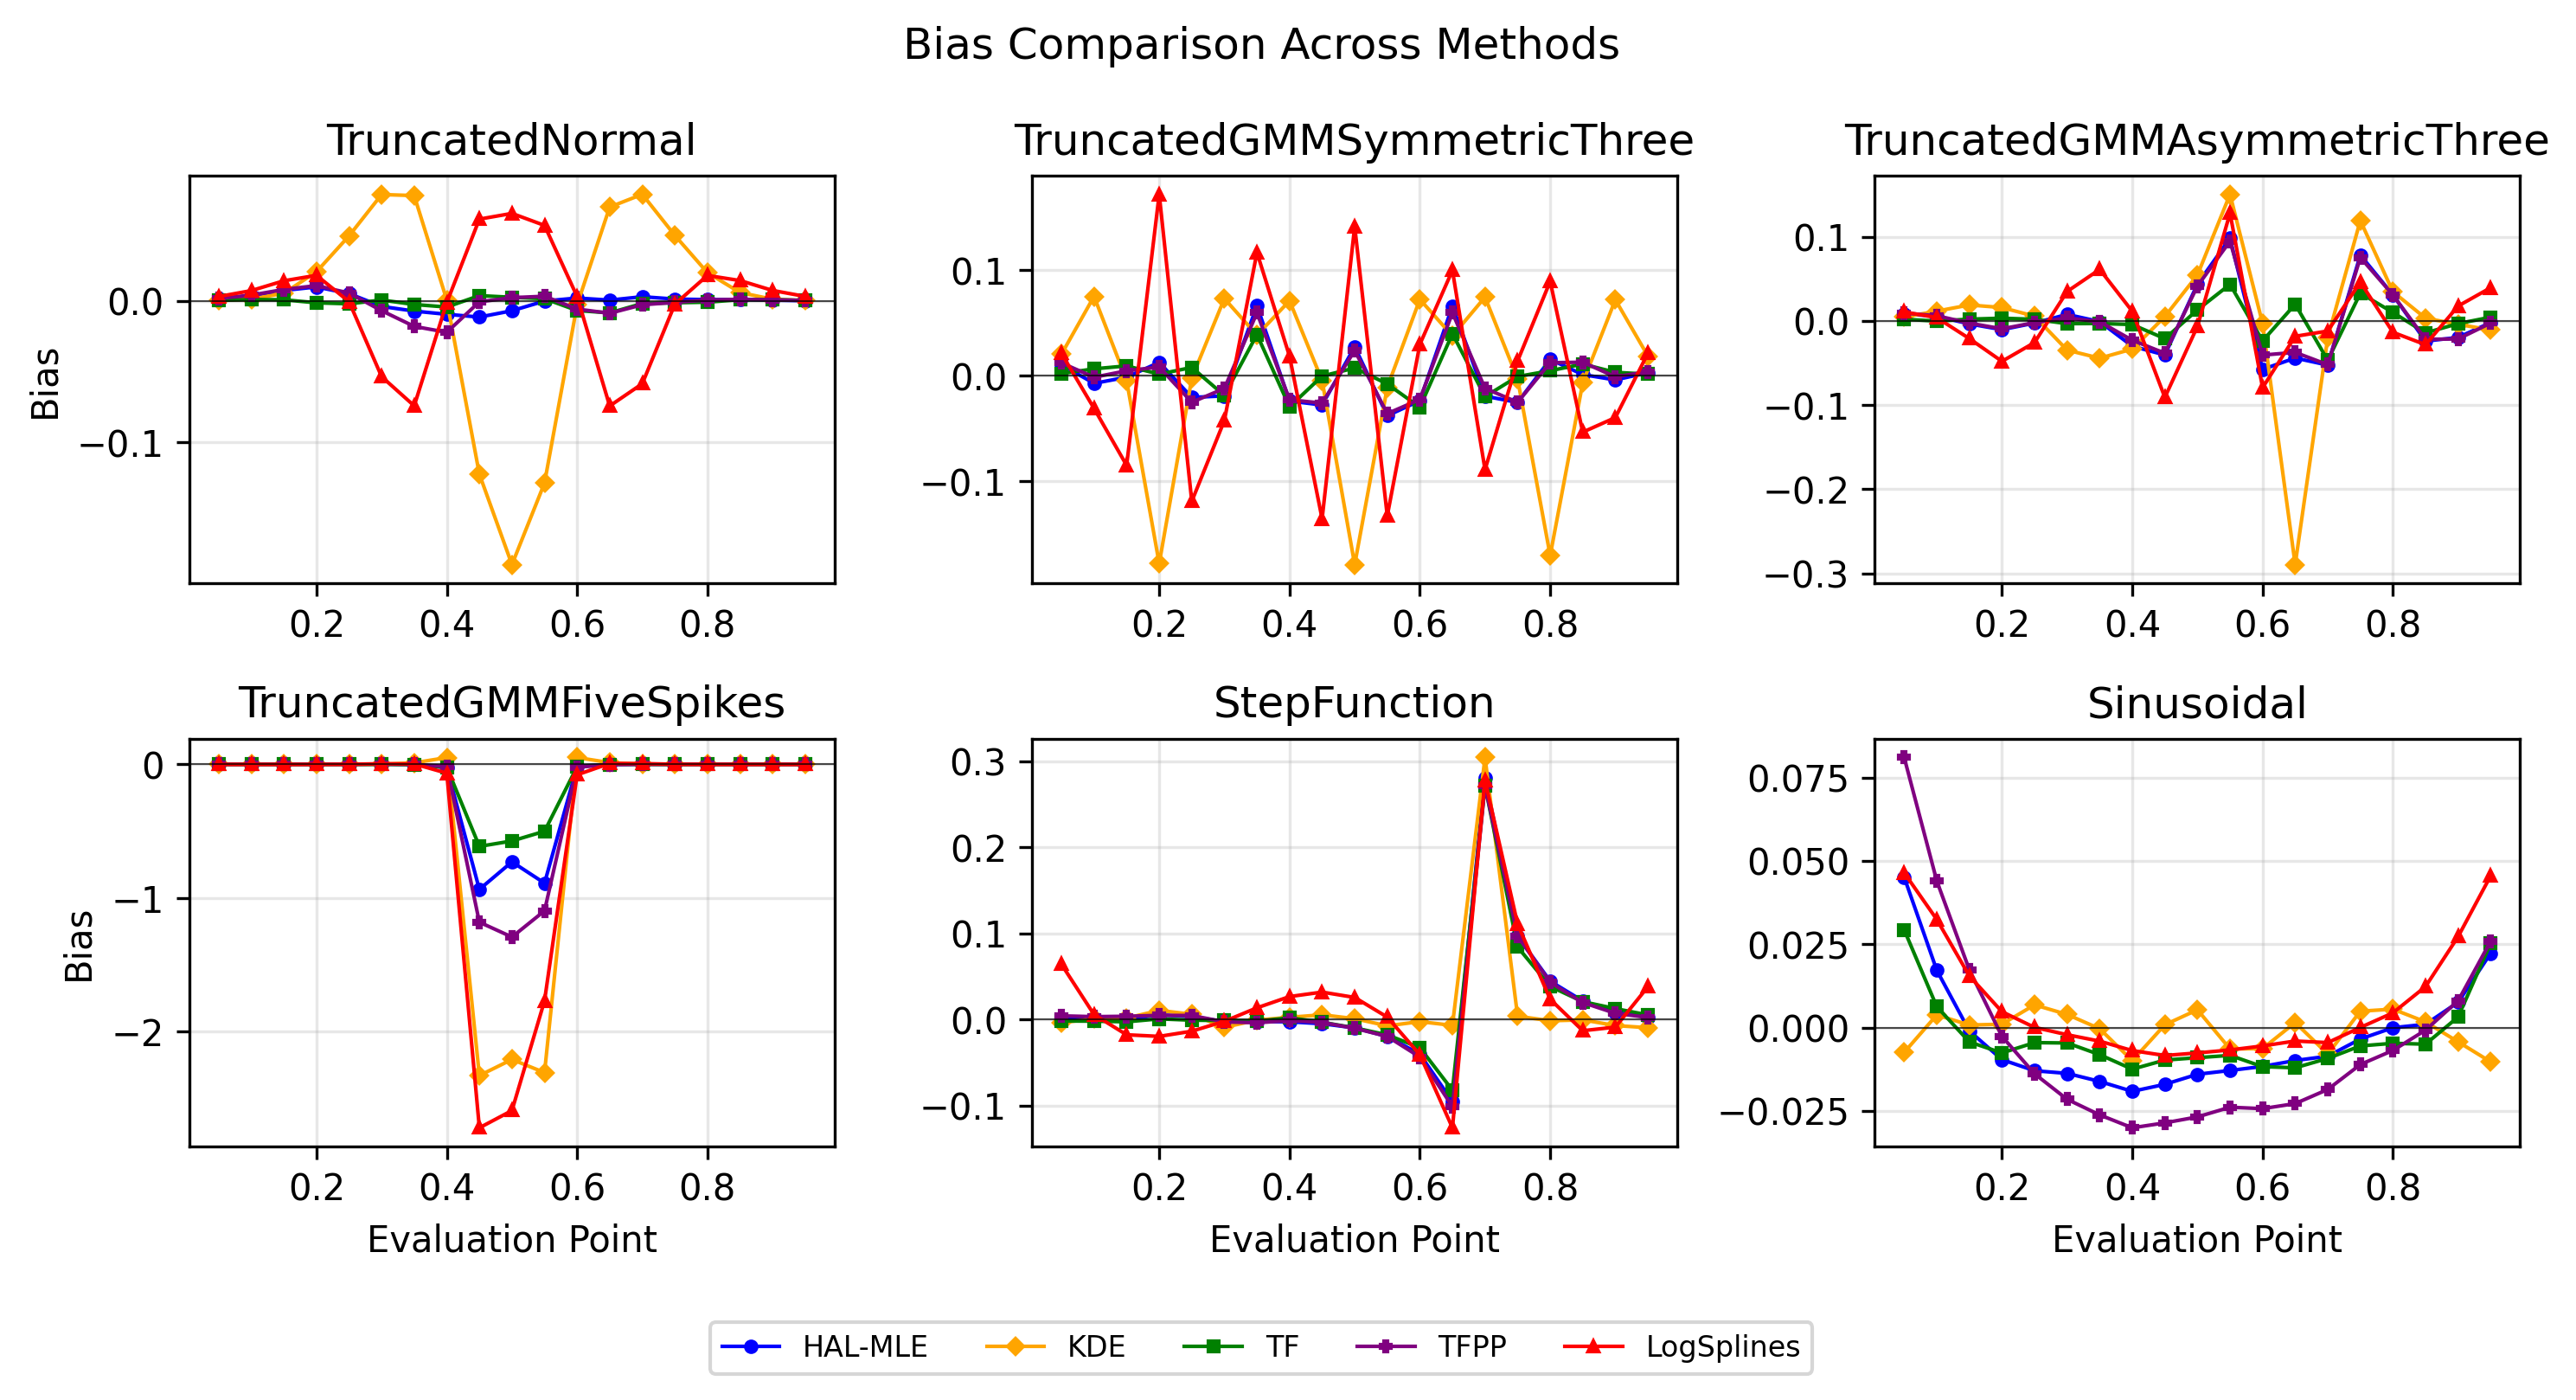
\includegraphics[width=\textwidth]{resources/density_bias_variance_mse_analysis/methods_compare_bias_across_dgps_N800.png}
    \caption{Bias at $n=800$ across six DGPs (columns) for five estimators (legend).}
    \label{fig:methods-bias-n800}
\end{figure}

\begin{figure}[H]
    \centering
    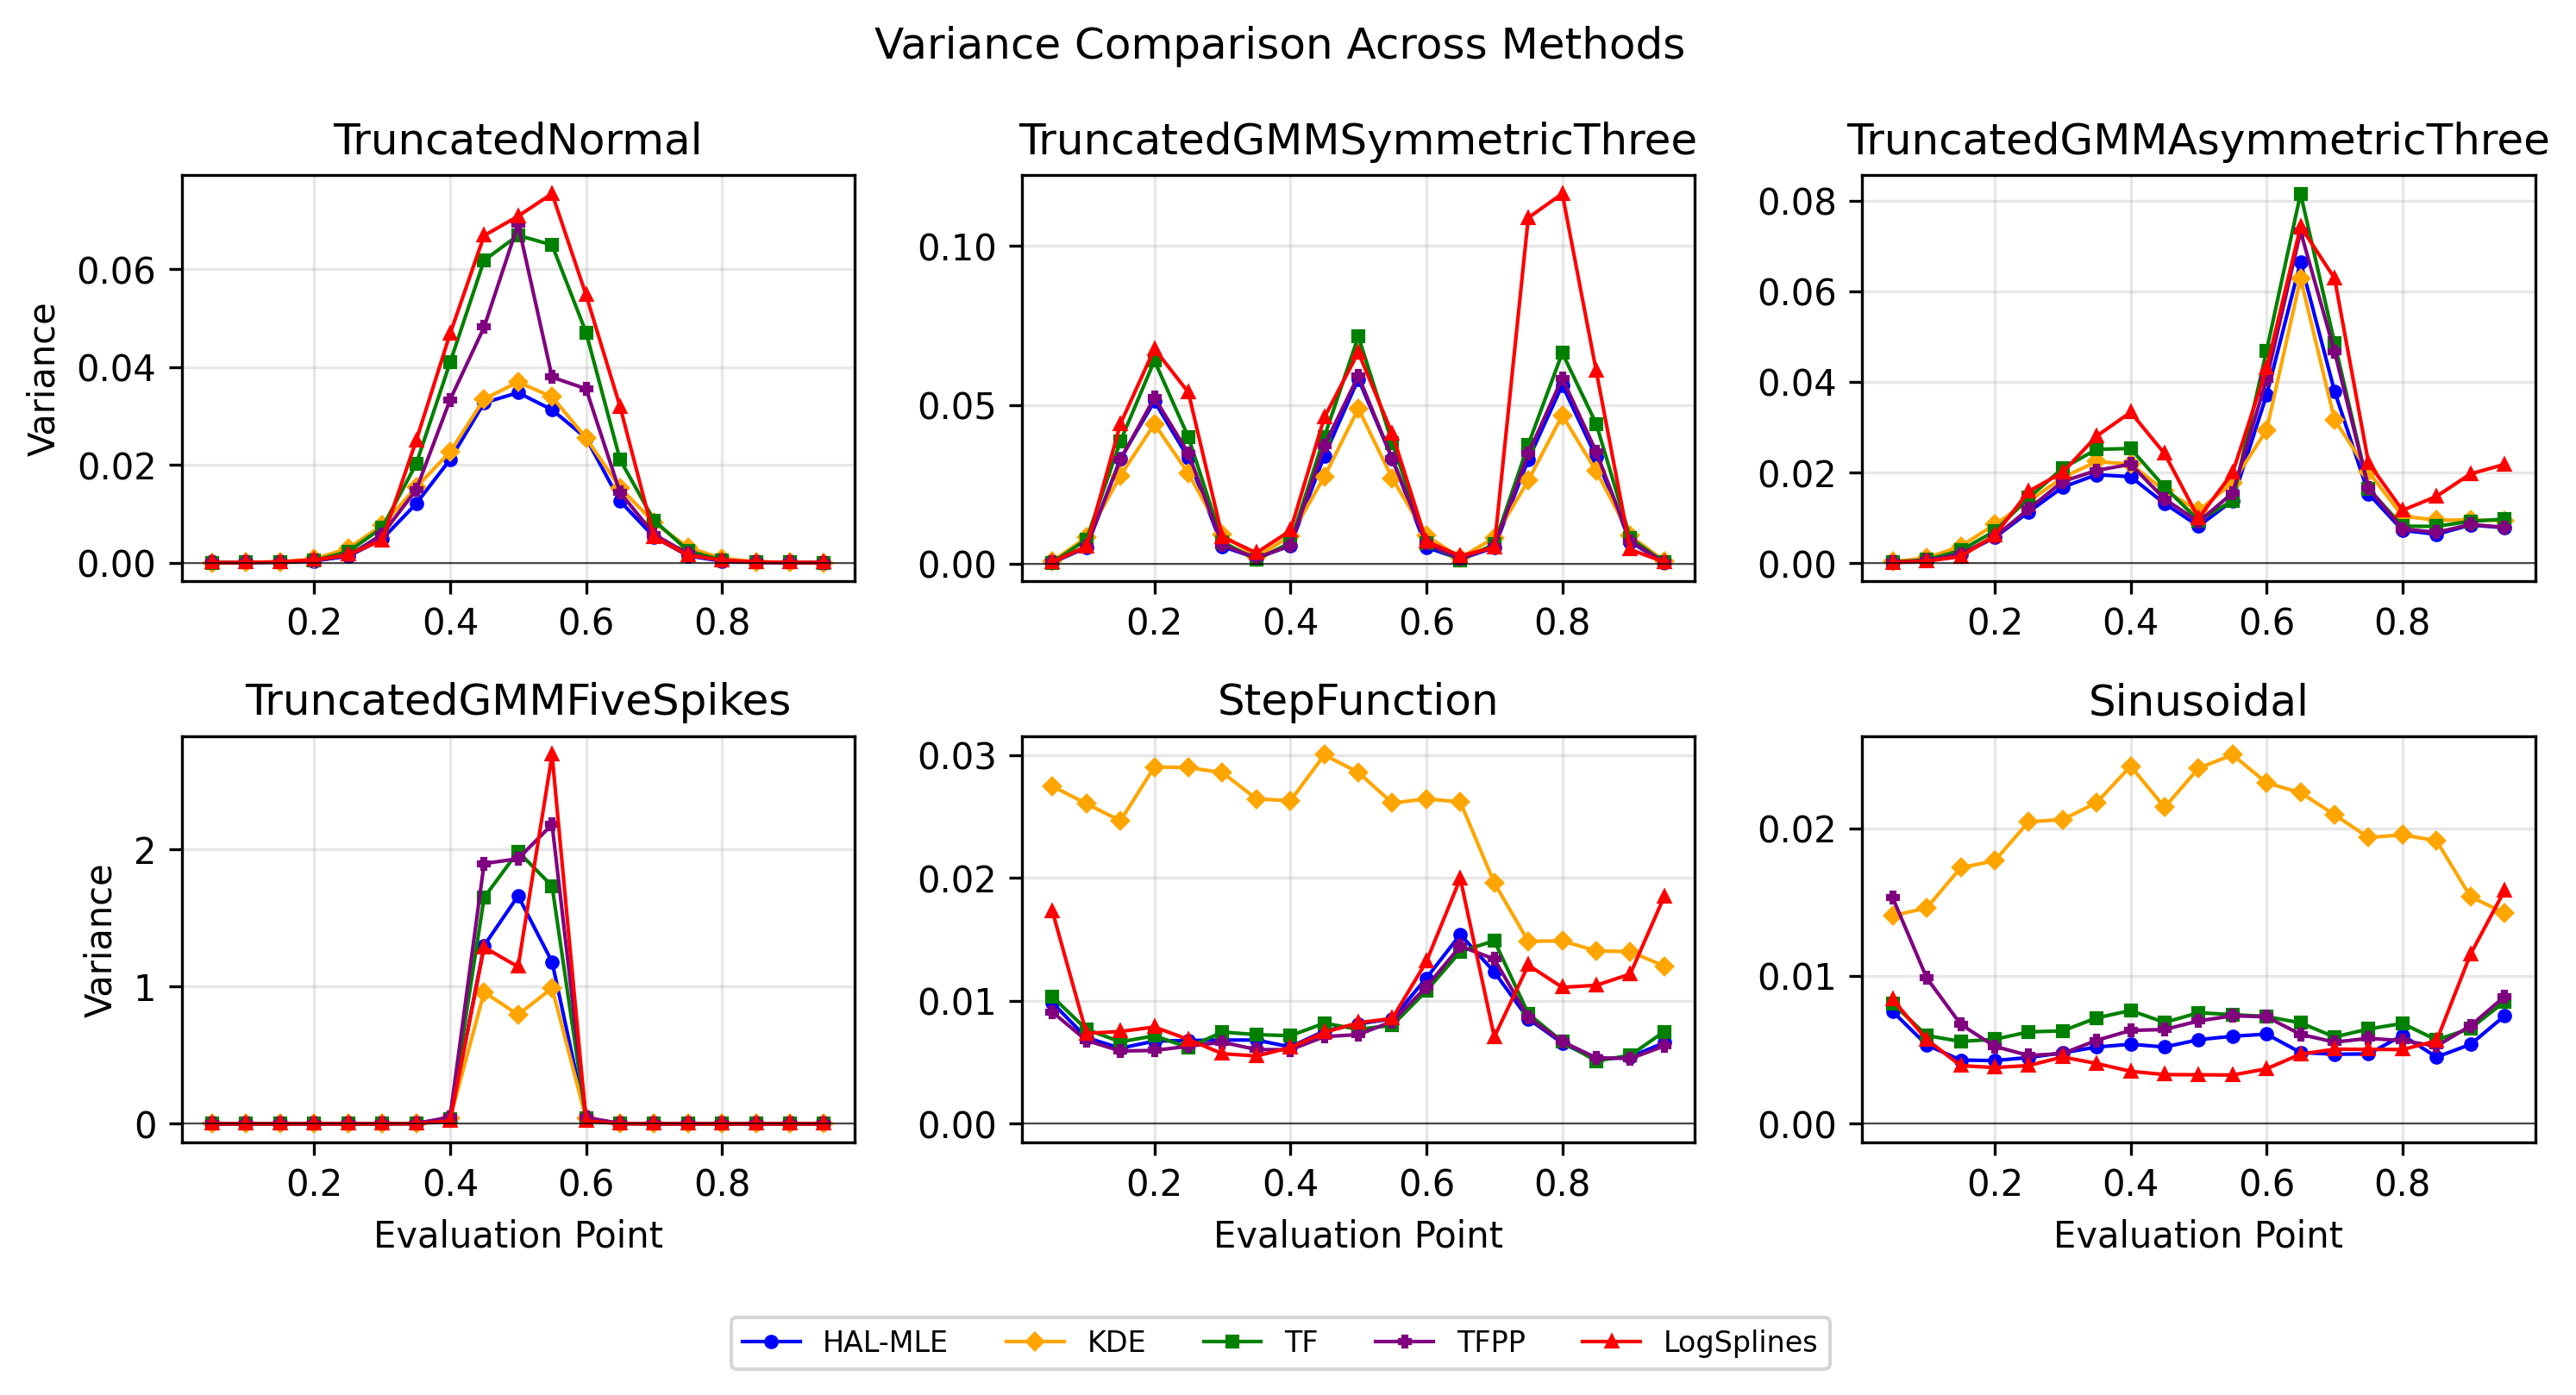
\includegraphics[width=\textwidth]{resources/density_bias_variance_mse_analysis/methods_compare_variance_across_dgps_N800.png}
    \caption{Variance at $n=800$ across six DGPs (columns) for five estimators (legend).}
    \label{fig:methods-variance-n800}
\end{figure}

\begin{figure}[H]
    \centering
    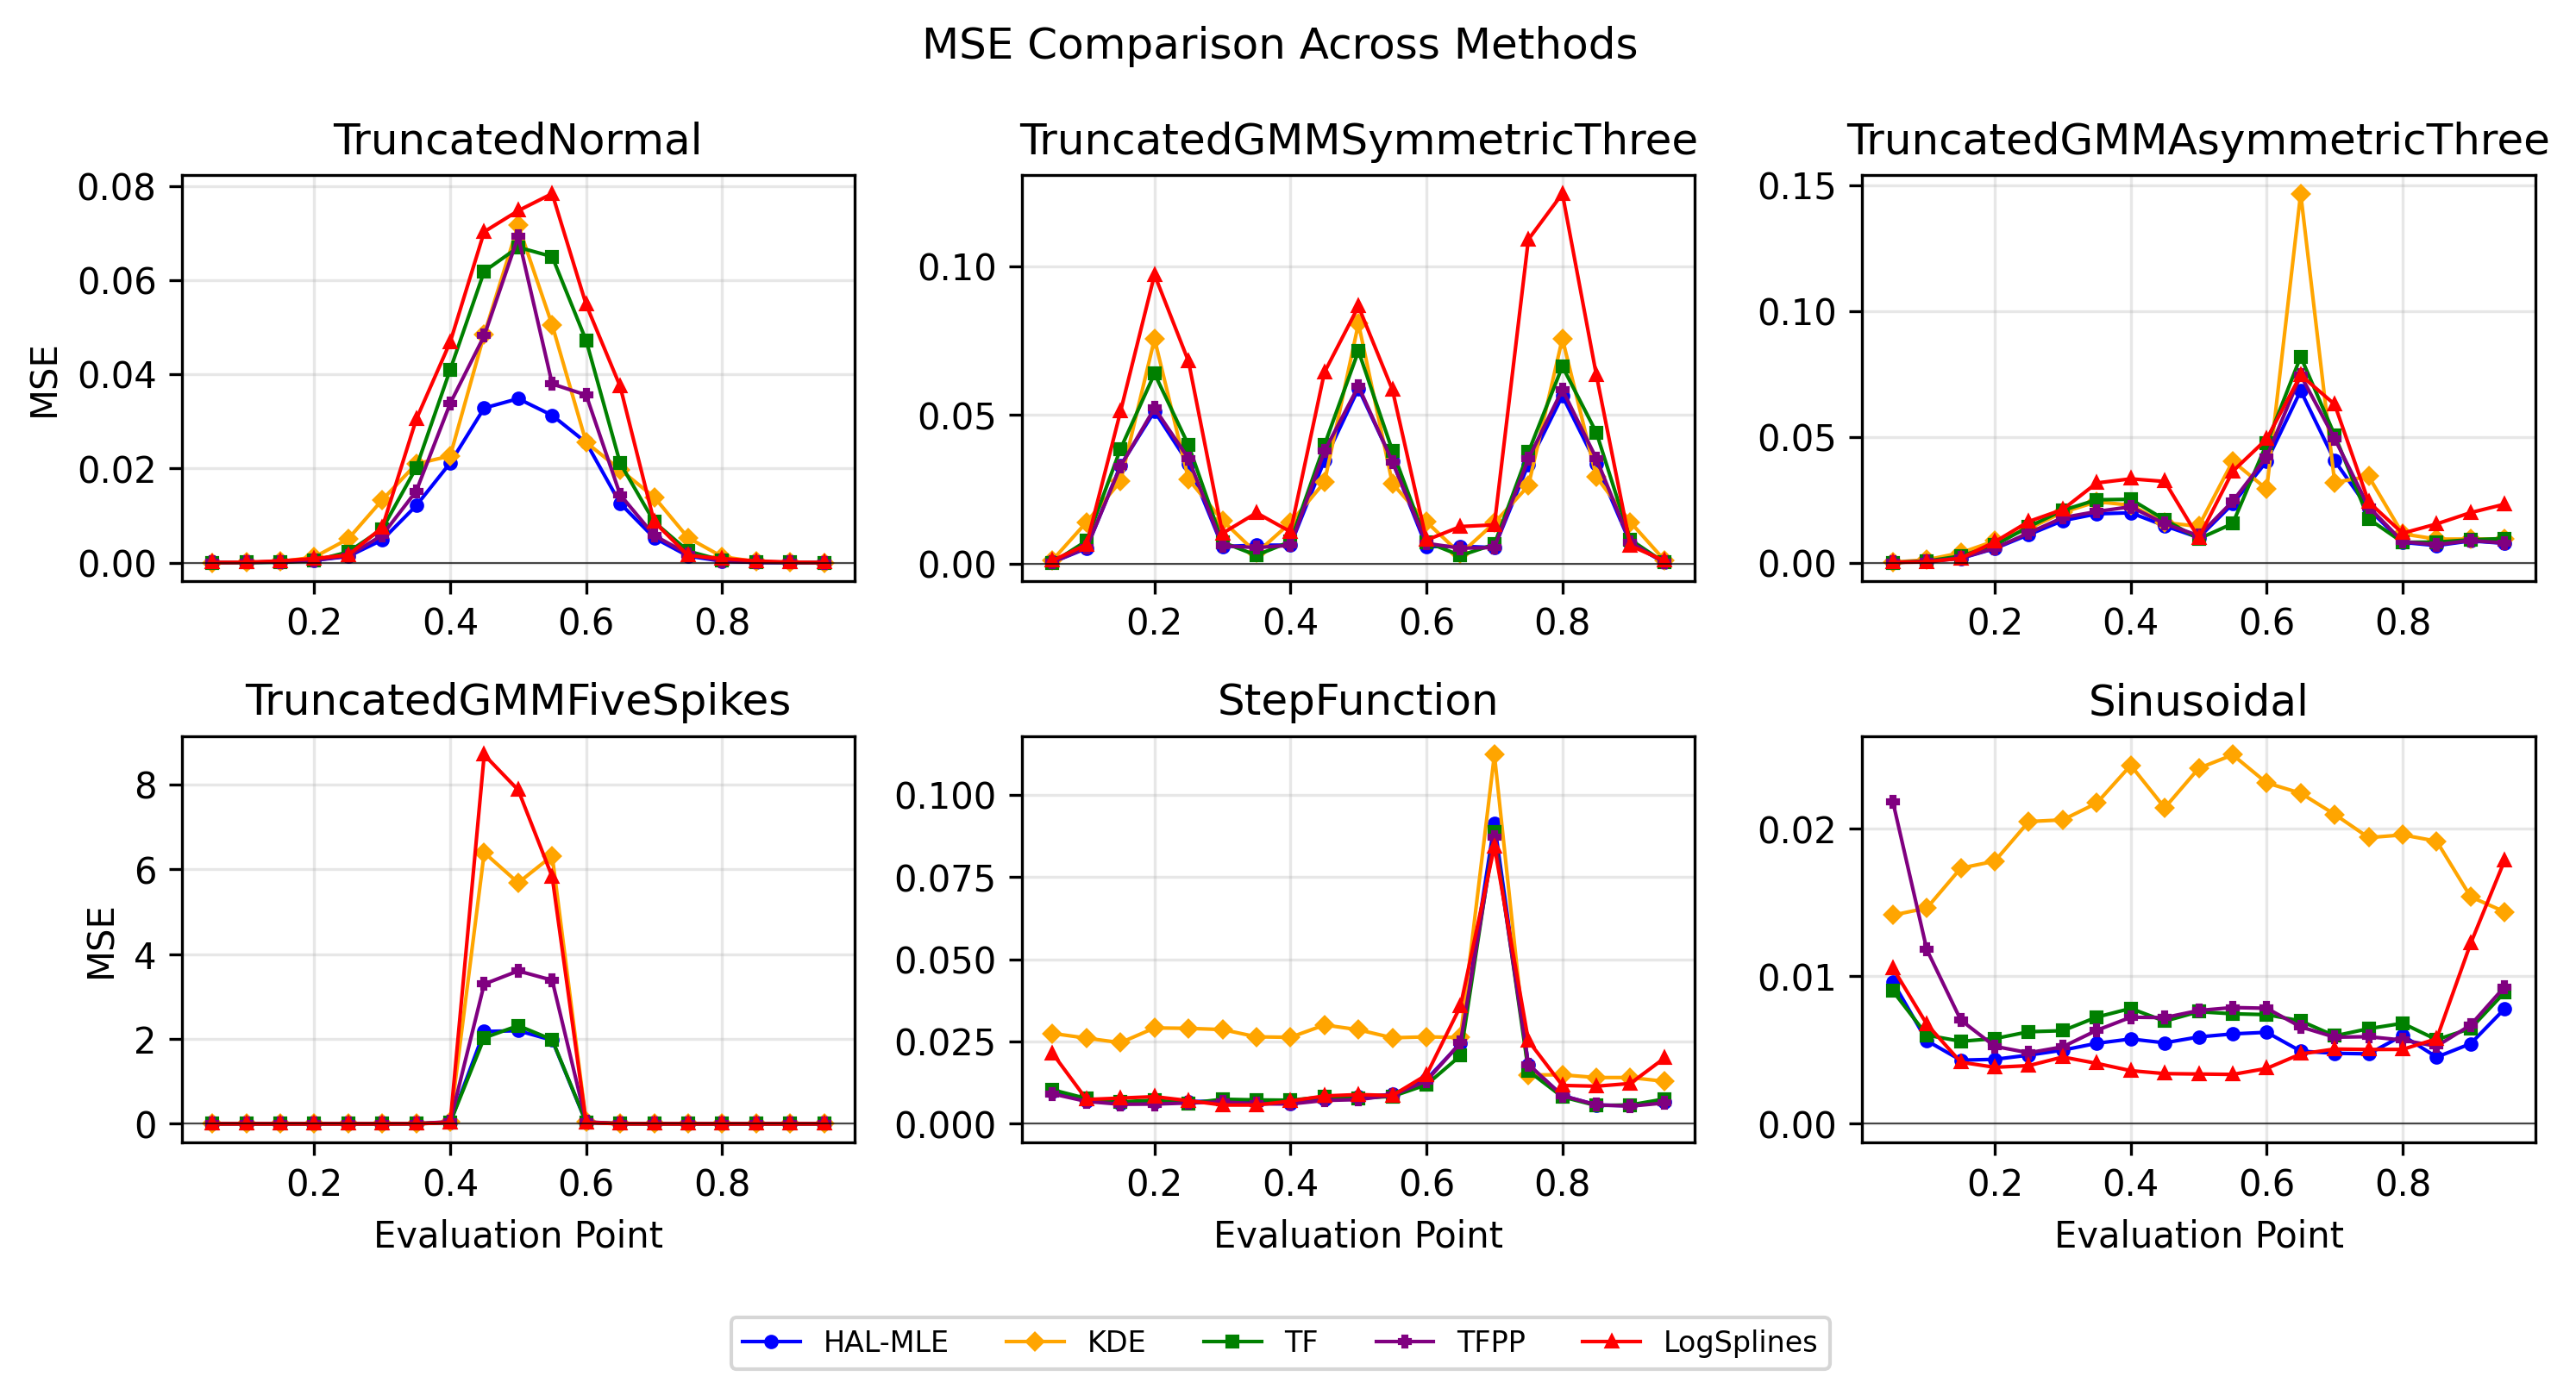
\includegraphics[width=\textwidth]{resources/density_bias_variance_mse_analysis/methods_compare_mse_across_dgps_N800.png}
    \caption{MSE at $n=800$ across six DGPs (columns) for five estimators (legend).}
    \label{fig:methods-mse-n800}
\end{figure}


Some observations of the comparison are as follows: (i) Comparing with logspline, which used the same link function but without controlling for the variation norm, the HAL-MLE is less biased and has a much lower MSE for the highly oscillatory DGPs, while preserving a slightly better performance on the other DGPs. (ii) Comparing with the KDE, the linear smoother, the HAL-MLE is less biased and has a much lower MSE and variance for the highly oscillatory, sudden change, and heavy-tailed DGPs. (iii) Comparing with the TF and TFPP, which controlled for the variation norm and the sectional variation norm respectively, but with a different basis system, the HAL-MLE are comparable in terms of bias and MSE. Theoretically, the 0th and 1st order falling factorial basis and the 0th and 1st order truncated power basis are equivalent \citep{tibshirani2022divided}, but the performance of TFPP and HAL-MLE here are comparable but not equivalent. One reason is that the implementation of TF(PP) uses the uniform knots instead of data-adaptive knots as in the HAL-MLE, even though using the data-adaptive knots is plausible as described in \cite{wang2014falling}. The second reason is that our implementation of TF as described in Appendix~\ref{app:tf_admm} deals with the normalizing constant brutally and thus the performance is not equivalent as expected. We acknowledge that more effort is needed, and it is beyond the scope of this paper. However, we do argue that the current implementation of TF and TFPP with uniform knots is the more computationally efficient than the HAL-MLE with a comparable performance. We verified that the divided difference matrix and its variant with penalty on the parametric part, as introduced in \cite{wang2014falling}, using uniform knots or data-adaptive knots, have better condition number than the truncated power basis respectively. The performance gives us the confidence of generalizing the pointwise asymptotic normality and uniform convergence properties of HAL-MLE to TF.
